\documentclass [8pt] {beamer}
\usetheme{Copenhagen}
\usepackage[utf8]{inputenc}
\usepackage[russian]{babel}
\usepackage{indentfirst}
\usepackage{graphicx}
\usepackage{hyperref}

\sloppy

\title[]{DevOps: его роль в современной разработке программного обеспечения}
\institute[]{СГУ}
\author{Устюшин Б. А.}
\date{2023}
\setbeamerfont{institute}{size=\huge}
\setbeamerfont{author}{size=\huge}
\setbeamerfont{date}{size=\huge}
\setbeamertemplate{caption}[numbered]

\begin{document}

\begin{frame}[plain]
     \huge
     \vfill
     \centering
     \begin{beamercolorbox}[sep=8pt,center,colsep=-4bp,rounded=true,shadow=true]{institute}
        \usebeamerfont{institute}\insertinstitute
     \end{beamercolorbox}

     {\usebeamercolor[fg]{titlegraphic}\inserttitlegraphic\par}

     \begin{beamercolorbox}[sep=8pt,center,colsep=-4bp,rounded=true,shadow=true]{title}
        \usebeamerfont{title}\inserttitle\par%
        \ifx\insertsubtitle\@empty%
        \else%
        \vskip0.25em%
        {\usebeamerfont{subtitle}\usebeamercolor[fg]{subtitle}\insertsubtitle\par}%
      \fi%     
     \end{beamercolorbox}%

     \vskip1em\par

     \begin{beamercolorbox}[sep=8pt,center,colsep=-4bp,rounded=true,shadow=true]{author}
        \usebeamerfont{author}\insertauthor
     \end{beamercolorbox}

     \begin{beamercolorbox}[sep=8pt,center,colsep=-4bp,rounded=true,shadow=true]{date}
        \usebeamerfont{date}\insertdate
     \end{beamercolorbox}\vskip0.5em

    \end{frame}

\section{Введение}
\begin{frame}
\huge

Сегодня мы:
\vskip0.25cm
\large

\begin{itemize}
\item Поймём, какие основные задачи у DevOps
\item Узнаем об основных инструментах, которыми пользуется DevOps
\item Рассмотрим вопрос безопасности и логирования при разработке ПО
\item Рассмотрим основные навыки DevOps инженера
\end{itemize}
\end{frame}

\subsection{Кто такой DevOps?}
\begin{frame}
\begin{columns}[T]
\column{0.4\textwidth}
\vskip2.2cm
\centering
\huge
Кто такой DevOps?
\column{0.6\textwidth}
\begin{figure}[H]
	\center{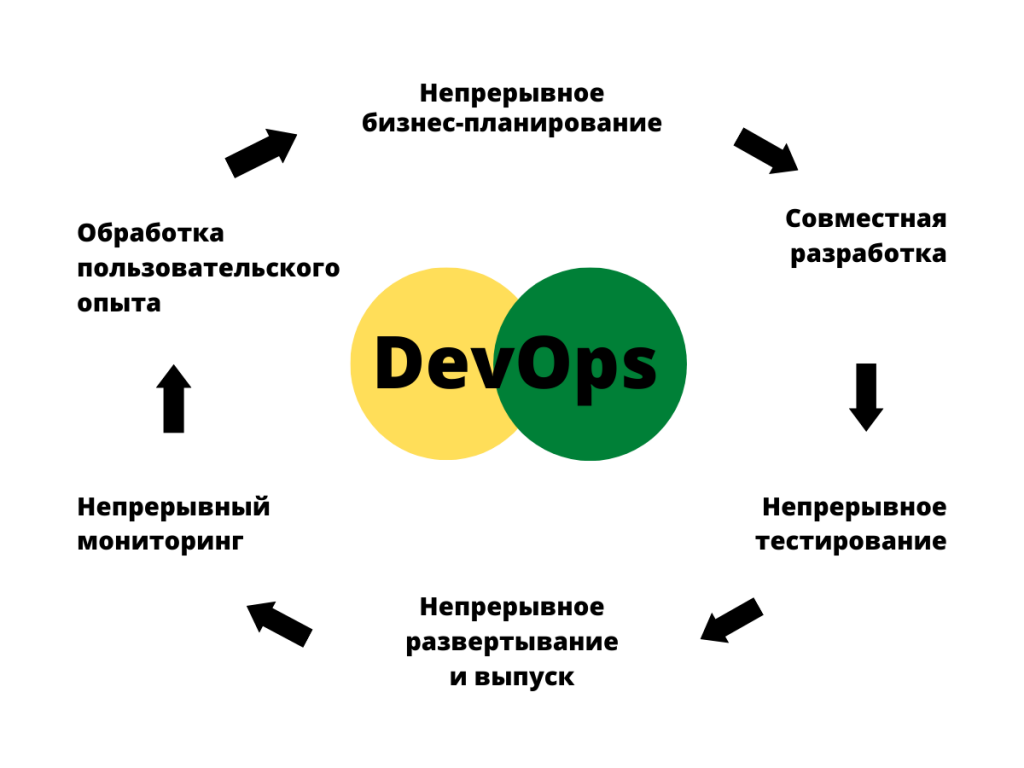
\includegraphics[scale=0.25]{img1.png}}
\end{figure}
\end{columns}
\end{frame}

\begin{frame}
\Huge

Основные задачи DevOps
\vskip0.25cm
\Large

\begin{enumerate}
\item Ускорение разработки приложений
\item Автоматизация процессов существования приложений
\item Упрощение работы основных разработчиков
\item Обеспечение безопасности работы приложения
\item Мониторинг данных о работе приложений
\end{enumerate}
\end{frame}

\section{Основные инструменты DevOps}
\subsection{Ускорение разработки}

\begin{frame}
\begin{columns}[T]
\column{0.7\textwidth}
\begin{figure}[H]
	\center{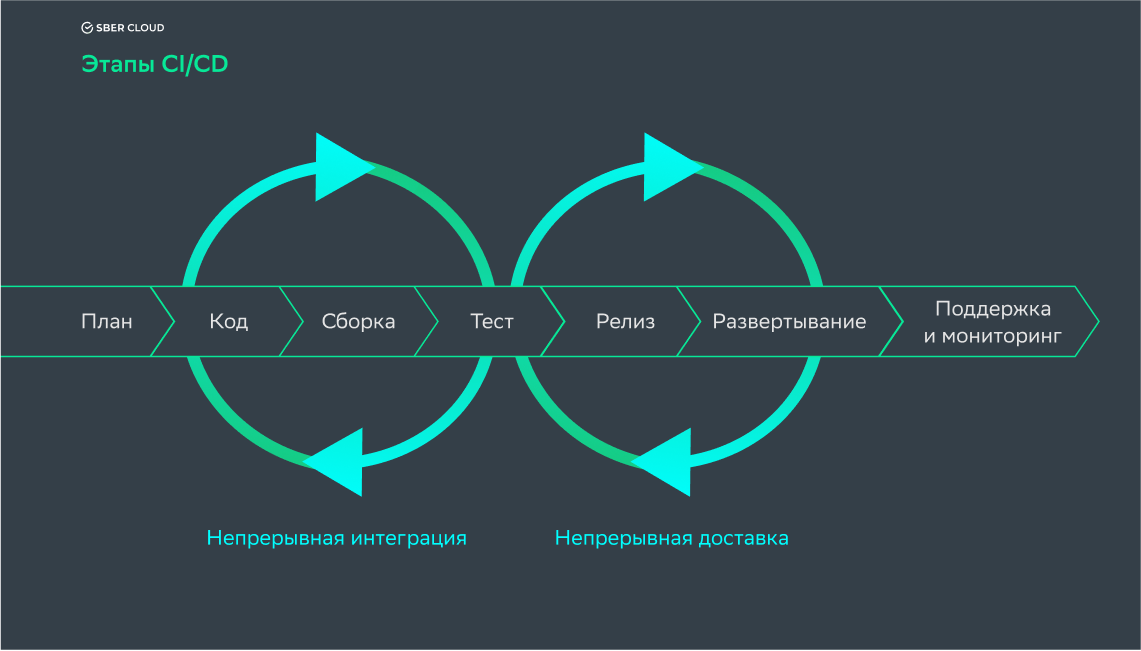
\includegraphics[scale=0.3]{img2.png}}
\end{figure}
\column{0.3\textwidth}
\vskip1.8cm
\centering
\huge
CI \\
CD
\end{columns}
\end{frame}

\begin{frame}
\begin{columns}[T]
\column{0.4\textwidth}
\vskip1.7cm
\centering
\huge
Git \\
Система контроля версий
\column{0.7\textwidth}
\begin{figure}[H]
	\center{
\includegraphics[scale=0.7]{img3.png}}
\end{figure}
\end{columns}
\end{frame}

\begin{frame}
\begin{columns}[T]
\column{0.7\textwidth}
\begin{figure}[H]
	\center{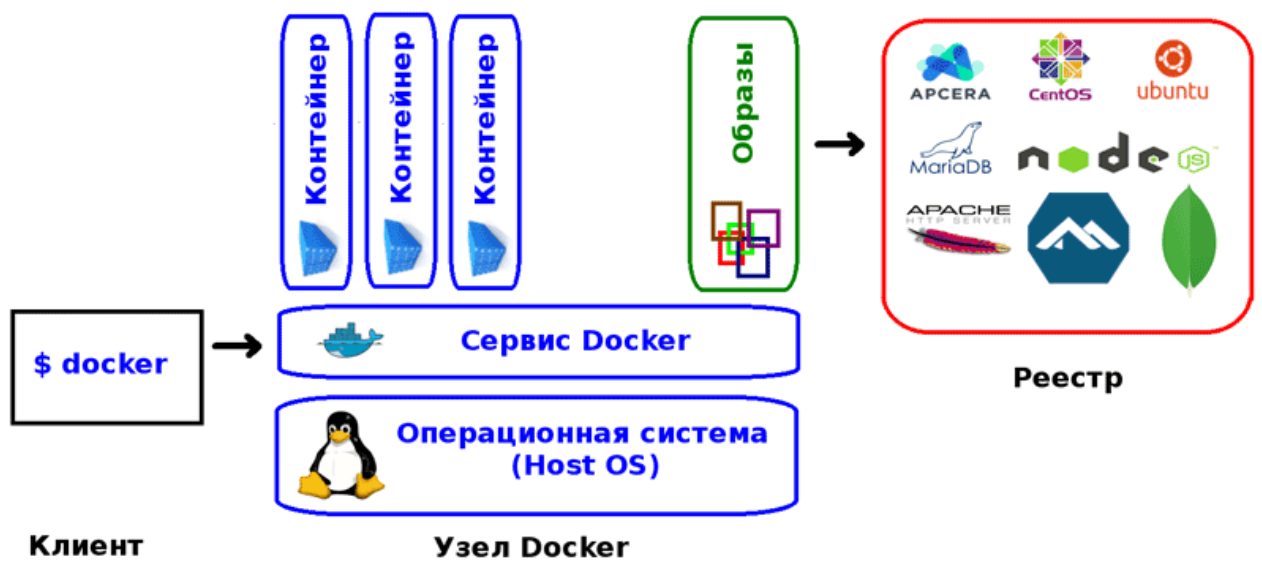
\includegraphics[scale=0.24]{img4.png}}
\end{figure}
\column{0.3\textwidth}
\vskip1.7cm
\centering
\huge
Docker
\end{columns}
\end{frame}

\begin{frame}
\begin{figure}[H]
	\center{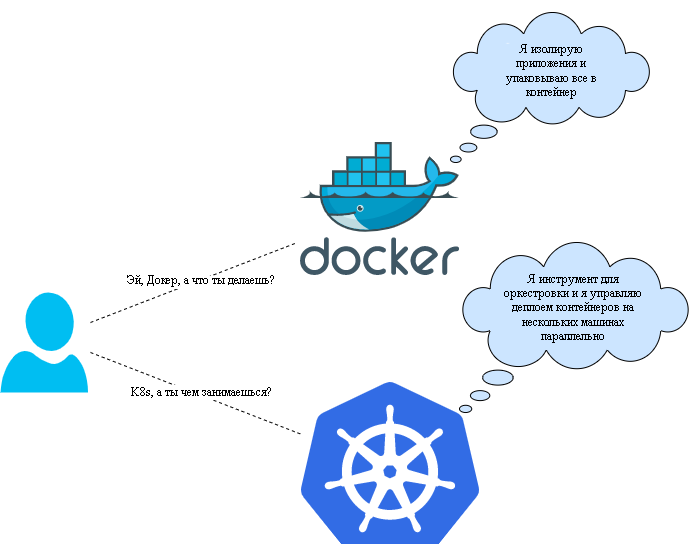
\includegraphics[scale=0.35]{img5.png}}
\end{figure}
\end{frame}

\begin{frame}
\Huge
\centering
ChatGPT
\vskip0.4cm

\begin{figure}[H]
	\center{
\includegraphics[scale=0.8]{img6.png}}
\end{figure}

\end{frame}

\section{Безопасность}

\begin{frame}
\Huge
\centering
Безопасность
\begin{columns}[T]
\column{0.65\textwidth}
\begin{figure}[H]
	\center{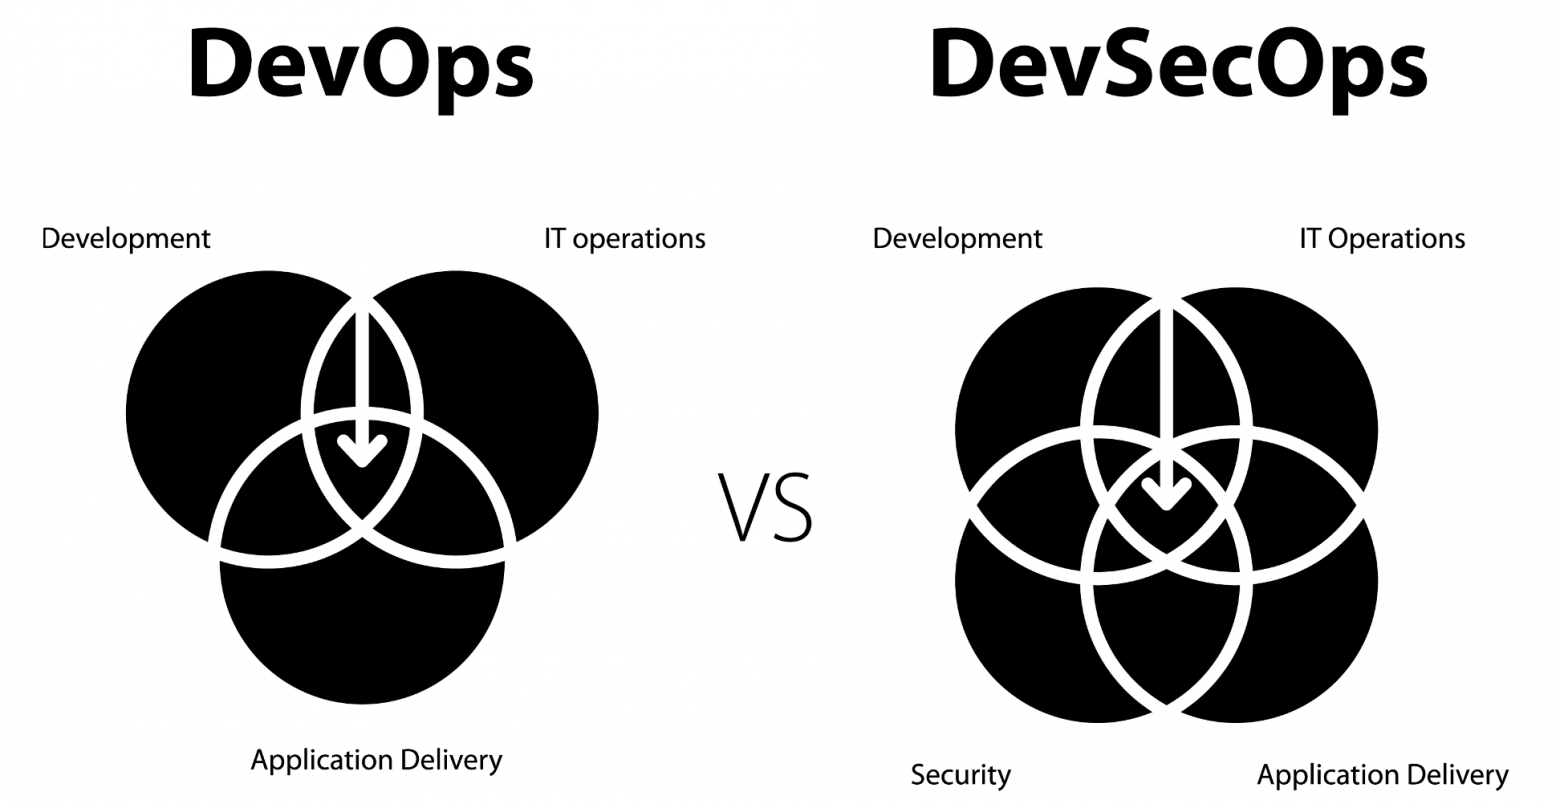
\includegraphics[scale=0.18]{img7_1.png}}
\end{figure}
\column{0.45\textwidth}
\vskip1cm
\begin{figure}[H]
	\center{
\includegraphics[scale=0.35]{img7_2.png}}
\end{figure}
\end{columns}
\end{frame}

\begin{frame}
\begin{columns}[T]
\column{0.2\textwidth}
\vskip2.4cm
\centering
\huge
Мониторинг
\column{0.8\textwidth}
\begin{figure}[H]
	\center{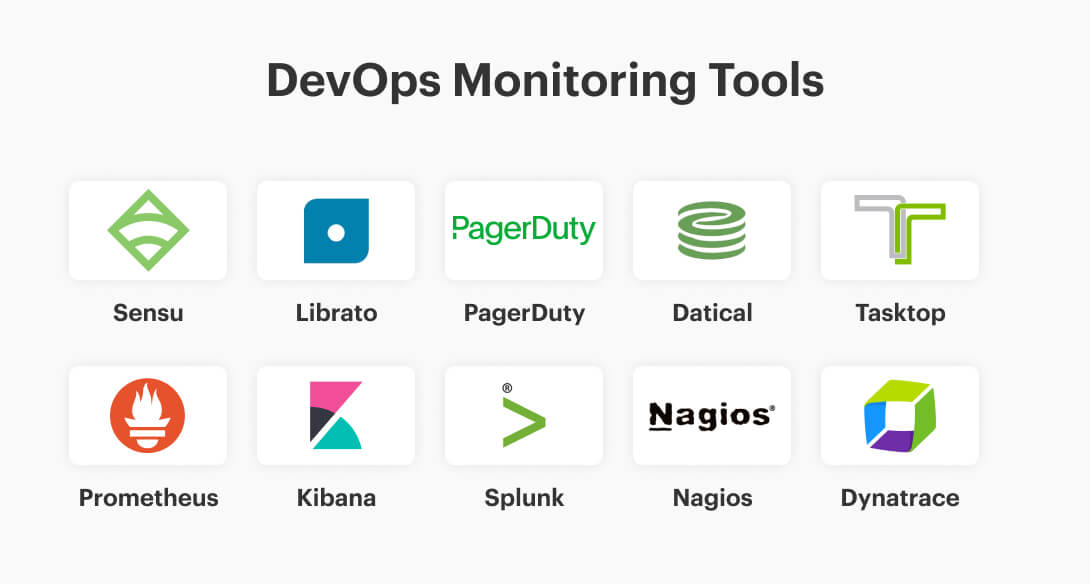
\includegraphics[scale=0.25]{img8.png}}
\end{figure}
\end{columns}
\end{frame}

\begin{frame}
\Huge
\centering
Качества DevOps-инженера
\vskip0.4cm

\begin{figure}[H]
	\center{
\includegraphics[scale=0.4]{img9.png}}
\end{figure}

\end{frame}

\begin{frame}
\begin{columns}[T]
\column{0.33\textwidth}
\vskip0.6cm
\begin{figure}[H]
	\center{
\includegraphics[scale=0.5]{fin2.png}}
	\caption{Количество вакансий в Москве}
	\label{fin2}
\end{figure}
\column{0.33\textwidth}
\begin{figure}[H]
	\center{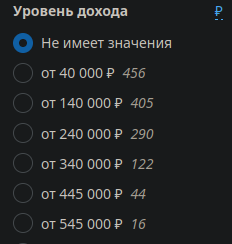
\includegraphics[scale=0.5]{fin1.png}}\
	\caption{Уровень дохода в Москве(из 2779 вакансий не у всех указан)}
	\label{fin1}
\end{figure}
\column{0.33\textwidth}
\vskip0.4cm
\begin{figure}[H]
	\center{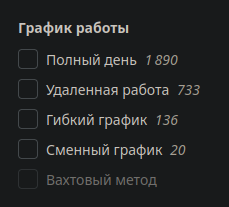
\includegraphics[scale=0.5]{fin3.png}}
	\caption{График работы в Москве}
	\label{fin3}
\end{figure}
\end{columns}
\end{frame}

\section{Заключение}

\begin{frame}
\Huge
\centering
Заключение
\end{frame}


\section{Ссылки на источники}
\large
\begin{frame}
\begin{thebibliography}{00}
\bibitem{} \href{URL: https://ru.wikipedia.org/wiki/Система_управления_версиями}{Система управления версиями, Википедия}
\bibitem{} \href{URL: https://habr.com/ru/companies/otus/articles/515078/}{Что такое CI/CD? Разбираемся с непрерывной интеграцией и непрерывной поставкой}
\bibitem{} \href{URL: https://selectel.ru/blog/what-is-docker}{Что такое Docker: для чего он нужен и где используется}
\bibitem{} \href{URL: https://habr.com/ru/articles/253877/}{Понимая Docker}
\bibitem{} \href{URL: https://strawpoll.com/most-popular-version-control-system}{Статистика популярности систем контроля версий}
\bibitem{} \href{https://kubernetes.io/ru/docs/concepts/overview/what-is-kubernetes/}{Что такое Kubernetes?}
\bibitem{} \href{URL: https://uk.indeed.com/viewjob?jk=7bd6b6bd58342cad&from=serp&vjs=3}{Вакансия Prompt-инженера}
\bibitem{} \href{URL: https://www.keepersecurity.com/ru_RU/resources/glossary/what-is-devops-security/}{Что такое безопасность DevOps?}
\bibitem{} \href{URL: https://proglib.io/p/12-instrumentov-devops-inzhenera-dlya-monitoringa-arhitektury-2020-02-13}{Инструменты для мониторинга архитектуры}

\end{thebibliography}
\end{frame}

\section{}

\Huge
\begin{frame}
\centering
Спасибо за внимание!
\end{frame}
\end{document}